\section{Introducción}

Luego de haber ayudado a Scaloni y el equipo técnico a ordenar los análisis de los siguientes rivales de la selección \textbf{CAMPEONA DEL MUNDO}, Scaloni planteó un cronograma de entrenamiento para los jugadores, pero se cruzó con un problema: no sabe qué días conviene entrenar y cuales descansar para que los jugadores tengan la mayor ganancia posible y puedan dar el mejor desempeño en el próximo mundial. Pero que no cunda el pánico, Menotti le recomendó usar una técnica que será la que nos ayudará a resolver este problema: \textit{"Programación Dinámica"}.

Ahora bien, ¿En qué consiste la \textit{Programación Dinámica}? Para entender esto, es necesario entender ciertos puntos:
\begin{itemize}
	\item Usa una técnica de optimización llamada \textit{Memoization} (memorización en inglés). Esta técnica se basa en guardar los resultados ya calculados de un problema para poder ser reutilizados más adelante sin ser necesario que se calculen nuevamente.
	\item El problema que se desea solucionar debe poder descomponerse en subproblemas que a su vez estos permitan construir las soluciones a problemas más grandes.
	\item La cantidad de subproblemas debe ser polinomial.
	\item Esta técnica nos permite reducir la complejidad temporal de un algoritmo, evitando explorar un espacio exponencial de soluciones.
\end{itemize}
Una vez planteado esto, lo que se refiere a la \textit{Programación Dinámica} es hacer uso de la \textit{Memoization} y guardar las soluciones de los subproblemas más pequeños para poder ir construyendo las soluciones cada vez más grandes hasta llegar a dar con la solución deseada. Pero para poder aplicar esta técnica, es necesario antes saber la forma que tienen los subproblemas y como estos se combinan para dar solución a un problema más grande.
Viendo por donde viene el asunto, se nos puede venir a la cabeza la \textit{recurrencia}, y esto es correcto ya que esta técnica se sustenta gracias al uso de este método, y la solución se hallara gracias a haber hallado la \textbf{\textit{Ecuación de Recurrencia}} del problema. Una vez obtenida, se puede plantear el problema iterativamente (en vez de hacerlo recursivo) pero siguiendo los principios de la técnica y hacer uso de la memorización. Hacerla de forma iterativa nos será de gran ayuda ya que es más fácil de entender qué es lo que está pasando y cuándo, y porque es mucho más fácil de calcular la complejidad.

En nuestro problema que se nos planteó, necesitamos saber que días conviene entrenar y cuáles no dependiendo de la ganancia obtenida del entrenamiento y la energía de los jugadores. Tener en cuenta lo siguiente:
\begin{itemize}
    \item Los entrenamientos son inamovibles. No podemos cambiar el entrenamiento $e_i$ con el entrenamiento $e_j$ ($i \neq j$).
	\item Para el dia del entrenamiento $e_i$, la energía disponible va a ser menor o igual a la del dia $e_{i-1}$, por lo tanto se cumple
	\[ s_1 \geq s_2 \geq ... \geq s_n \]
	siendo estas las energías disponibles para cada $e_i$ después de haber entrenado consecutivamente. La energía $s_1$ corresponde al día $e_1$.
	\item Si se descansa un dia, el primer dia de volver a entrenar vuelve a tener la energía del primer dia.
	\item Si el valor del entrenamiento del día $e_i$ tiene valor $j$, y la energía disponible para ese dia es $s_i$, la ganancia será del mínimo de estos dos. Es decir,
	\[ Ganancia(i) = min(j, s_i) \]
\end{itemize}
Entonces teniendo en mente lo anterior mencionado, nuestros subproblemas serían proporcionales a la cantidad de días que hayan programado. A su vez, la forma de estos subproblemas es calcular el óptimo del día \texttt{i} dependiendo de si conviene haber entrenado o no el día anterior y tener en cuenta la ganancia de este día. La forma en la que los subproblemas se combinan para dar lugar a la solución de los problemas más grandes es a través de, una vez calculado los \textit{óptimos} de los días hasta \textit{i-1} y teniendo en cuenta descansos y sus ganancias, para el dia \textit{i} la solucion seria hacer uso de la memorización de lo ya calculado y elegir la mejor opcion segun la \textbf{\textit{Ecuación de Recurrencia}} de nuestro problema.

Para definir nuestra ecuación de recurrencia, planteamos lo siguiente:
\begin{itemize}
	\item Para el primer día, la ganancia va a ser el mínimo entre la energía de ese día y el valor del entrenamiento.
	\item Para el segundo dia va a depender de si conviene haber entrenado el primer día y obtener la ganancia del entrenamiento como si fuera el primer dia de haber entrenado o continuar entrenando después del primer dia pero \textbf{no} con la energía que tendrían disponible los jugadores si hubieran descansado.
	\item Para el entrenamiento $e_i$, el optimo seria el que maximiza la ganancia entre haber entrenado el dia $e_{i-1}$ y tener menos energía disponible para obtener la ganancia de ese dia, o no haber entrenado el día anterior y tener la posibilidad de obtener mas ganancia teniendo más energía disponible.
\end{itemize}

Entonces teniendo todo esto en mente, nuestra ecuación de recurrencia tendría la siguiente forma:

\begin{figure}[H]
    \centering
    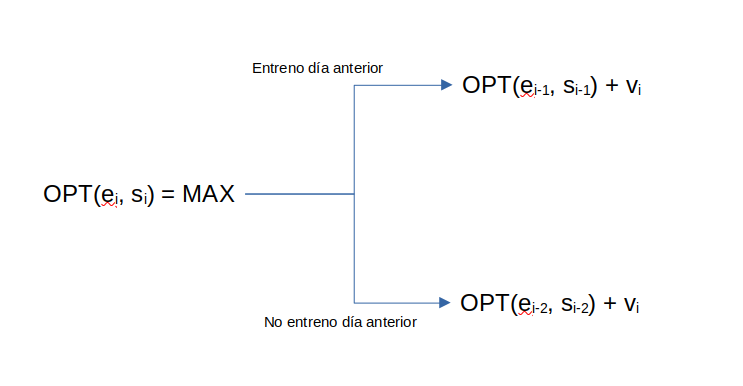
\includegraphics[width=0.9\textwidth]{img/equation.png}
\end{figure}

Consideraciones a tener en cuenta:

\begin{itemize}
	\item $v_i$ hace referencia al valor de la ganancia de ese día, que será el mínimo entre $s_i$ y $e_i$, los valores de energía y entrenamiento de ese día respectivamente.
	\item La opción de no entrenar el dia anterior solo es válida cuando estamos en el óptimo de $s_1$, ya que este corresponde a tener toda la energía disponible por haber descansado el día anterior.
	\item La opción de entrenar el dia anterior es válida cuando me encuentro en un $s_i$ donde $i$ es mayor a 0, ya que estará entrenando en el $i$ día seguido.
	\item Tendremos dos casos bordes:
	\begin{enumerate}
    	\item En el dia $1$ no habrá días anteriores, por lo que la única posible ganancia de ese día estará dada por el valor de $v_1$.
    	\item En el dia $2$, ya que no tendra dos días atrás para ver la ganancia de dicho dia. Entonces sus únicas dos posibilidades del óptimo es no haber entrenado el día $1$ y tener la ganancia del mínimo entre $e_2$ y $s_1$, o haber entrenado el día anterior y tener el optimo como indica la ecuación.
	\end{enumerate}
\end{itemize}
